\documentclass{beamer}
\usepackage[english]{babel}
\usepackage[utf8]{inputenc}
\usepackage[T1]{fontenc}
\usepackage{lmodern}
\usepackage{hus-beamer}
\usepackage{ifthen}
\usepackage[bibstyle=authoryear, citestyle=authoryear, maxcitenames=2, maxbibnames=2, backend=bibtex]{biblatex}
%\usepackage[maxbibnames=2]{biblatex}
%citestyle=authoryear or numeric or ...
\addbibresource{ref.bib}

%------ tikZ ------%
\usepackage{tikz}
\usetikzlibrary{tikzmark,overlay-beamer-styles,babel} 
\usetikzlibrary{positioning, arrows}
\usetikzlibrary{backgrounds}
    
\mode<presentation>{
	\usefonttheme{professionalfonts} % normal font for math formulas
	% insert section page with title only
	% before each section
	\AtBeginSection[]{
	\begin{frame}%[noframenumbering] % remove this if you do not want to number section page
	\vfill
	\centering
	\begin{beamercolorbox}[sep=8pt,center,shadow=true,rounded=true]{title}
	\usebeamerfont{title}\insertsectionhead\par%
	\end{beamercolorbox}
	\vfill
	\end{frame}
}
}

\begin{document}
\title{Improving Performance}
%\subtitle{Week 4}
\author{COMP6252 (Deep Learning Technologies)}
\institute[ECS, University of Southampton]{ECS, University of Southampton}
 \date{}

\begin{frame}
	\frametitle{Residual Networks}
\begin{itemize}
	\item Better results in image classification/recognition tasks when using deeper models 
	\item Can one keep adding layers  to get better results ?
	\item Initially deeper models faced the vanishing/exploding gradient problem
	\item That was solved using normalization techniques
	\item Another problem appeared when adding many layers: \textit{degradation of accuracy}
	\item Not caused by overfitting: \textbf{training} accuracy is degraded 
\end{itemize}
\end{frame}

\begin{frame}
    \frametitle{Training/test error}
\begin{center}
    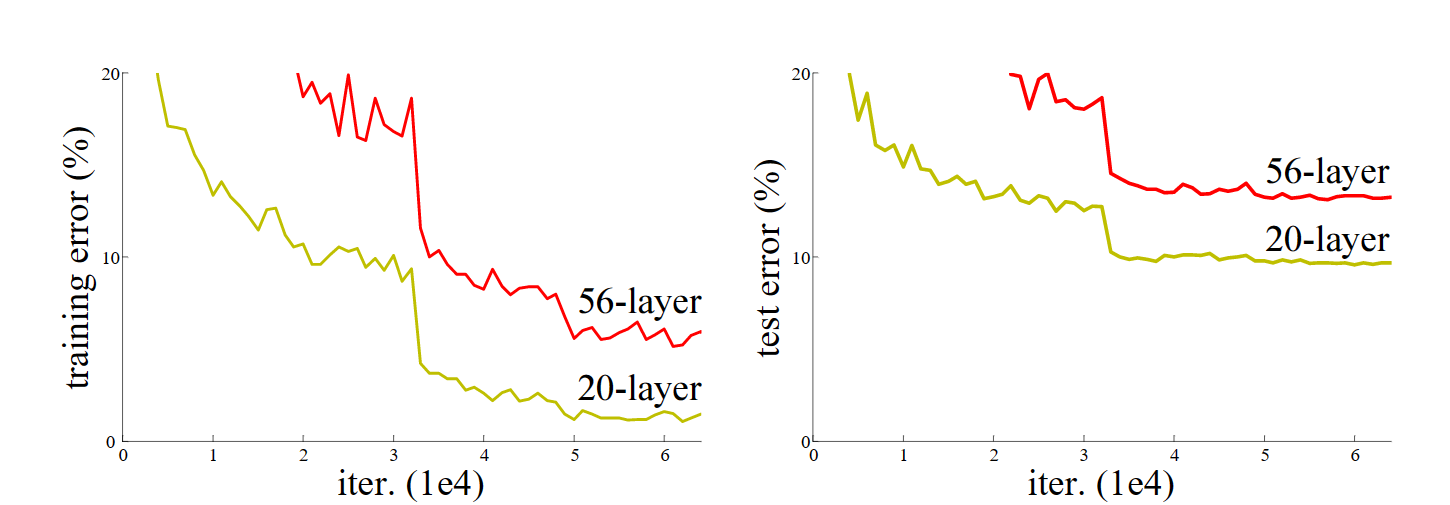
\includegraphics[width=\textwidth]{figs/deeper-error.png}
\end{center}

\end{frame}

\begin{frame}
    \frametitle{Basic problem}
\begin{itemize}
    \item Consider a model $M$ of depth $d$
    \item Construct a deeper model $N$ which adds a single layer $I$ to $M$
    \item With $I(x)=x$ the identity map
    \item Basically the output of $M$ is used as input to $L$
    \item The above implies that $N$ should not give higher error than $M$
    \item It turns out it is hard to learn the identity map
\end{itemize}
\end{frame}
\begin{frame}
    \frametitle{Learning the identify map}

\begin{itemize}
    \item Consider a convolutional layer followed by a ReLU,$\sigma$
    \item Given an input $x$ we can write
    \begin{align*}
        y=\sigma(conv(x))
    \end{align*}
    \item Can one find a kernel such that
    \begin{align*}
        x=\sigma(conv(x))
    \end{align*}
     \item  Regardless of the output $conv(x)$, for $x<0$ the above equation cannot be satisfied 
\end{itemize}    

\end{frame}
\begin{frame}
    \frametitle{Basic idea}
\begin{itemize}
    \item What about learning the zero map?
    \item If the desired map to be learned is $\mathcal{H}(x)$
    \item Define $\mathcal{F}(x)=\mathcal{H}(x)-x$
    \item Now if a component learns $\mathcal{F}(x)$
    \item All we have to do is add $x$ to the output
    \item This is done by adding a \textbf{skip} connection or a \textbf{shortcut}
\end{itemize}

\end{frame}
\begin{frame}
    \frametitle{Residual module}

    \begin{center}
        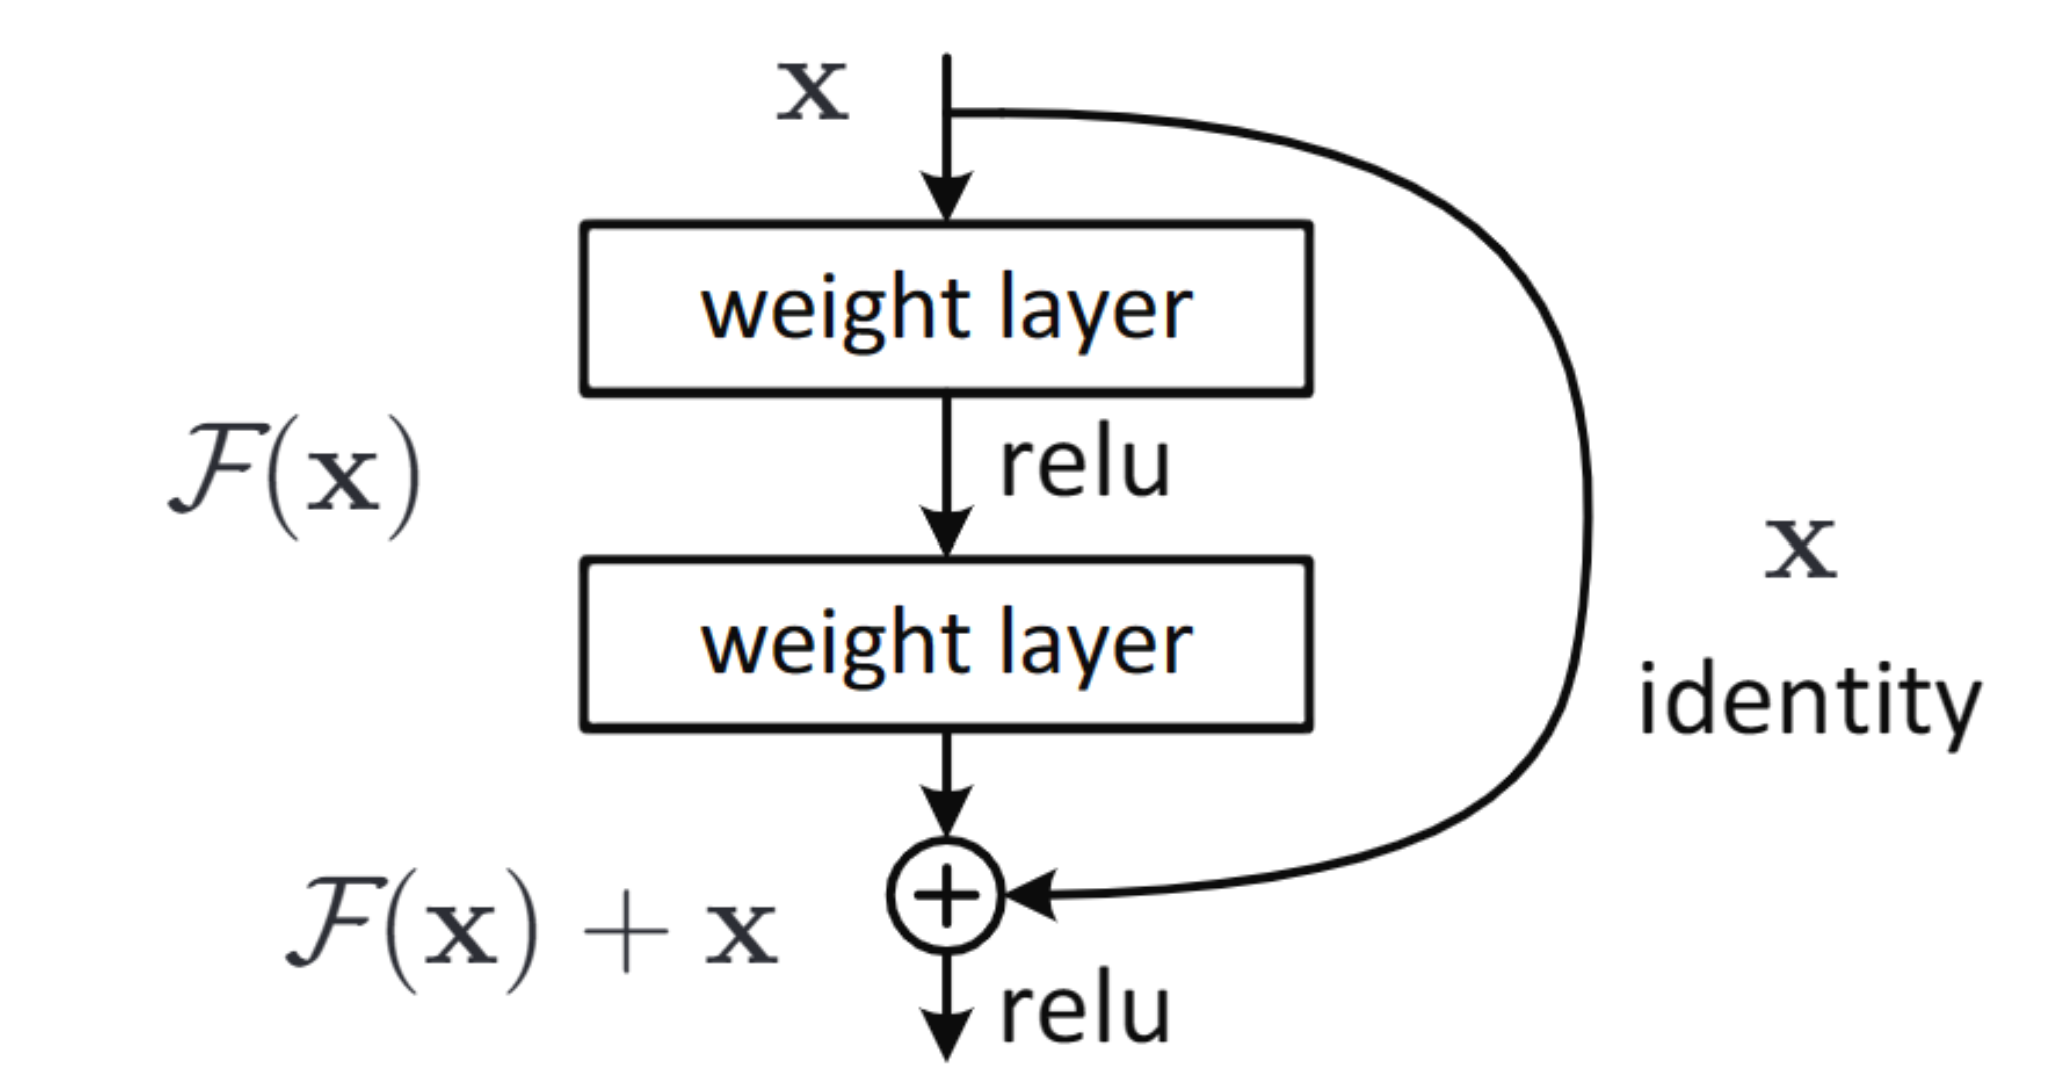
\includegraphics[width=\textwidth]{figs/residual-block.png}
    \end{center}
\end{frame}
\begin{frame}
    \frametitle{Resnet 34}

    \begin{center}
        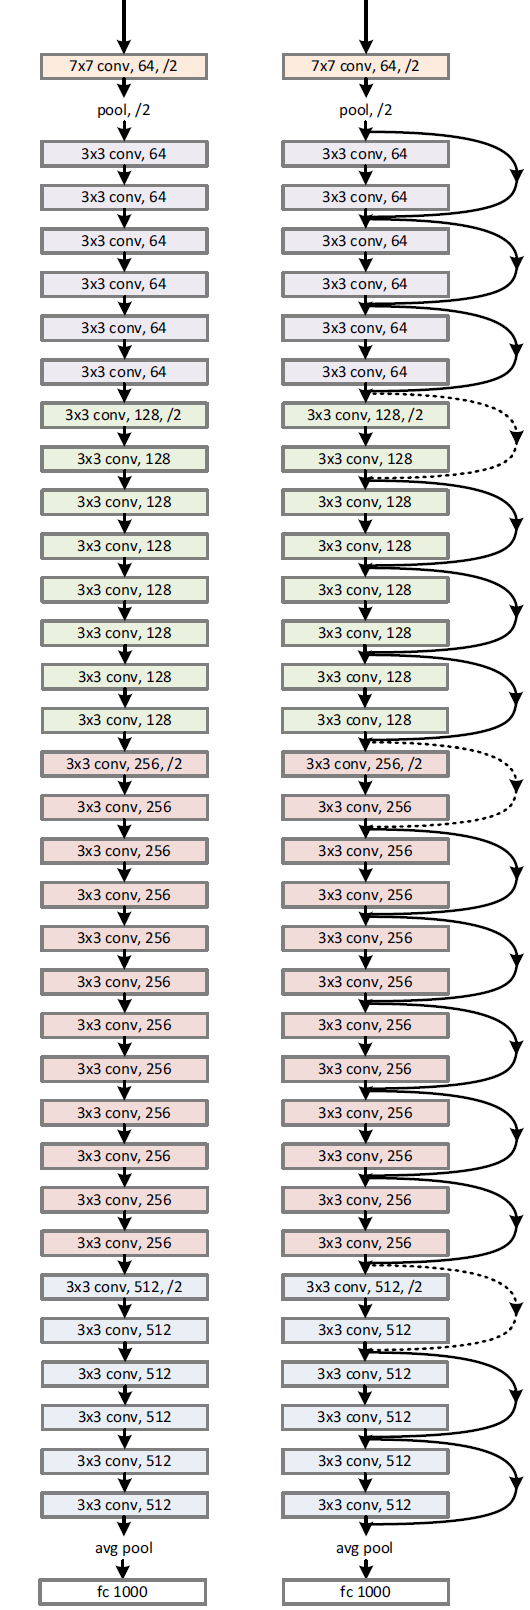
\includegraphics[width=0.22\textwidth]{figs/resnet34.png}
    \end{center}

\end{frame}
\end{document}